It is very cheap nowadays to produce data and many people are doing it due to technological advancement. Just as an example, in the field of genomics, the sequencing of the first human genome (2002) took around 13 years and cost over \$3 million to complete. Now we can sequence hundreds of genomes in a few days\cite{big_biological_impacts_bd}. This leads to the accumulation of vast quantities of genomic data, which can be used for new scientific discoveries, diagnose of rare diseases, etc. However we still need a human expert to visually inspect the data to find new signals and discover interesting patterns or to set a diagnosis. No matter how much resources we use into extracting the data if we don't get anything interesting out of it\cite{zhang_paciorkowski_craig_cui_2019}.

Some of the main problems that researchers face when analysing genomic data are: information overload, data interconnectivity and high dimensionality. One way to deal with all this data is to invent novel analysis. However, we still need visual inspection of the data, which is an important challenge, and this is what we attempt to solve. For this reason, it is very important to implement efficient visualization technologies that can lead to find new patterns and the extraction of good conclusions of the data. In the field of system biology, there are usually network representations where the nodes or bioentities are connected to each other and where these edges represent associations. Networks can increase dramatically in size and complexity and this is due to computational power to create very large networks, scientific knowledge about large networks and the big amounts of data that we have to analyze. We need better visualization systems for the analysis and inspection of networks and at the same time we need robust applications that can handle the data overload.

In Figure \ref{fig:network_biology_evolution} we can see a representation of the evolution for visualization of networks in system biology. Before the computers, networks were represented in 2 dimensions and they were static representations that lacked interactivity, see Figure \ref{fig:network_biology_evolution} A. With the computer era and the advancement in computer graphics, 3D representations were possible, with the addition of interactions (See Figure  \ref{fig:network_biology_evolution} C). As computer science progressed, visualization improved and also new technologies emerged like virtual reality, which has a huge potential with regards to the interactivity (Figure \ref{fig:network_biology_evolution} I).

\begin{figure}[h!]
    \newlength{\tempheight}
    \setlength{\tempheight}{15ex}
    \centering%
    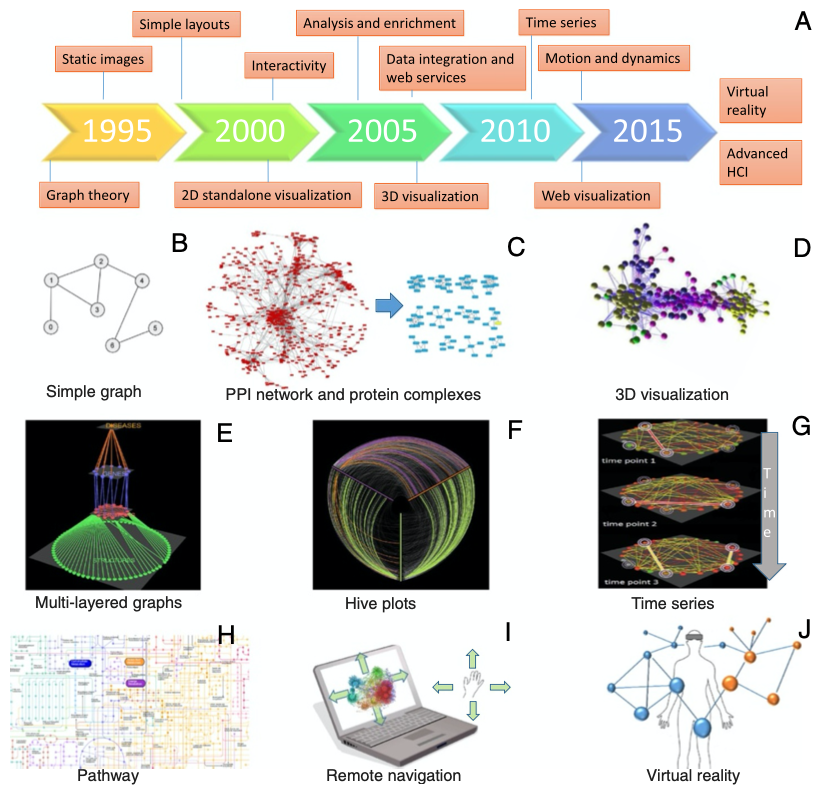
\includegraphics[width=\textwidth]{evolution_visualization}
    \caption{Visualization for network biology. a Undirected unweighted graph showing co-expression relationship between genes. b A 2D representation of a yeast protein-protein interaction network visualized in Cytoscape (left) and potential protein complexes 3D identified by the MCL algorithm from that network (right). c A 3D network of genes showing co-expression relationships. d A multilayered network integrating different types of data visualized by Arena3D. e A hive plot view of a network where nodes are mapped to and positioned on radially distributed linear axes. f Visualization of network changes over time. g Static picture showing part of lung cancer pathway. h Navigation of networks using hand gestures. i Integration and control of 3D networks using VR devices. Figure adapted\cite{pavlopoulos_malliarakis_papanikolaou_theodosiou_enright_iliopoulos_2015}.}
    \label{fig:network_biology_evolution}
\end{figure}%

We believe that virtual reality (VR) can offer new possibilities for visual inspection in large networks and for the inspection of patterns in these. Even though VR is still a field under exploration, it has been demonstrated that it help scientists work more effectively in fields like medicine \cite{Laver11}\cite{xia_ip_samman_wong_gateno_wang_yeung_kot_tideman_2001}\cite{brain_damage_rehab}, biology\cite{10.1093/bioinformatics/bti581}\cite{thorley_lawson_duca_shapiro_2008} and neuroscience\cite{bohil_alicea_biocca_2011}\cite{minderer_harvey_donato_moser_2016}, to  cite some examples. VR can be very powerful because it takes advantage of the way the human being perceives and analysis things. We have a great ability to discover patterns; however, we are biologically optimized to see the world and the patterns in 3 dimensions. Some of the advantages that VR has over non-VR approaches are the following:

\begin{enumerate}
  \item View of the environment in 3 dimensions and the possibility to move around the virtual space as in real life, giving a feeling of immersion.
  \item Interaction with the the environment by using hand controllers or the hands themselves, giving the user a feeling of presence.
  \item Possibility to combine 2-dimensional interfaces within the 3-dimensional virtual world that the user can interact with.
\end{enumerate}

We have implemented GeneNet VR, a virtual reality application for the visualization of 3-dimensional networks of genetic data. We have used up-to-date virtual reality techniques that we believe improve the visualization of this type of data structures. The techniques that we have used consist on: exploration of the network by moving around the virtual space, making it easier for the user to see the network from different perspectives; interaction with the network and the nodes to comprehend better the data and its associations; and the use of 2-dimensional user interfaces to manipulate the data for a easier pattern finding.

We saw that some of the interactions in GeneNet VR could have more impact in the performance of the application. This problem could escalate when using larger datasets. A high performance solution is desired so that pattern exploration in the network is not affected and novel patterns can be found in the networks.

\textbf{Thesis statement: } \emph{Virtual Reality techniques can be useful for the visualization of abstract networks and for the exploration of patterns in them}.

\section{Challenges and research problem}
It can be hard to identify novel patterns when visualizing large amounts of data. Some data structures, like the data networks, also have the challenge of data interconnectivity. These type of data structures represent relationships and are composed by nodes and edges. Even though we have many tools like machine learning, that help researchers automatize and accelerate the pattern recognition process, many times we still need a human expert to inspect these networks\cite{network_expert}.

In fields like biology, network visualization seem to be particularly helpful\cite{pujana_network_modeling}\cite{fraser_view_function}. There are many types of relationships that can be measure in a biological context, for example interactions between proteins or genetic interections when revealed by combinations of mutations. All these interactions and correlations can be easier to visualize as a network\cite{merico_visualization}.

MIxT\cite{fjukstad_dumeaux_olsen_lund_hallett_bongo_2017} is a web application for bioinformaticians that was used to identify genes and pathways in the primary tumor that are tightly linked to genes and pathways in the systemic response of a patient with breast cancer\cite{dumeaux_fjukstad_interactions_tumor_blood}. Among other tools, it offers a network visualization of genes which are represented as nodes and edges that represent statistically significant correlation in expression between the nodes.

When exploring a network in MIxT, sometimes it can be difficult to find patterns because of the data overload. This problem happens expecially when there are many nodes and relationships together. In figure \ref{fig:mixt_network} we can see an example of the network visualization from MIxT. As we can see in Figure \ref{fig:mixt_network1}, there are many nodes and relationships; this problem gets worse when we zoom in the network as in Figure \ref{fig:mixt_network_zoom}.

\begin{figure}[h!]
    \centering%
    \begin{subfigure}[t]{0.5\textwidth}
        \centering%
        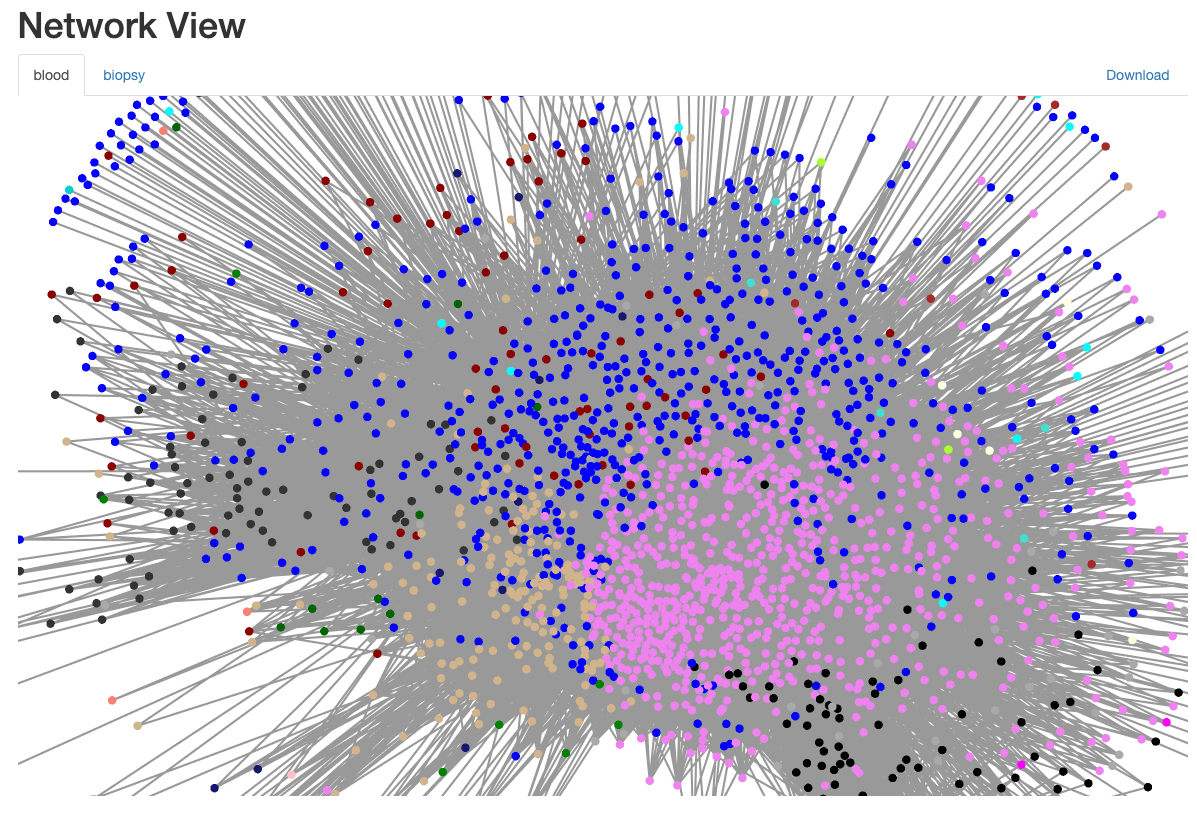
\includegraphics[width=\linewidth]{mixt_network1}
        \caption{Network with several modules.}
        \label{fig:mixt_network1}
    \end{subfigure}%
    \begin{subfigure}[t]{0.5\textwidth}
        \centering%
        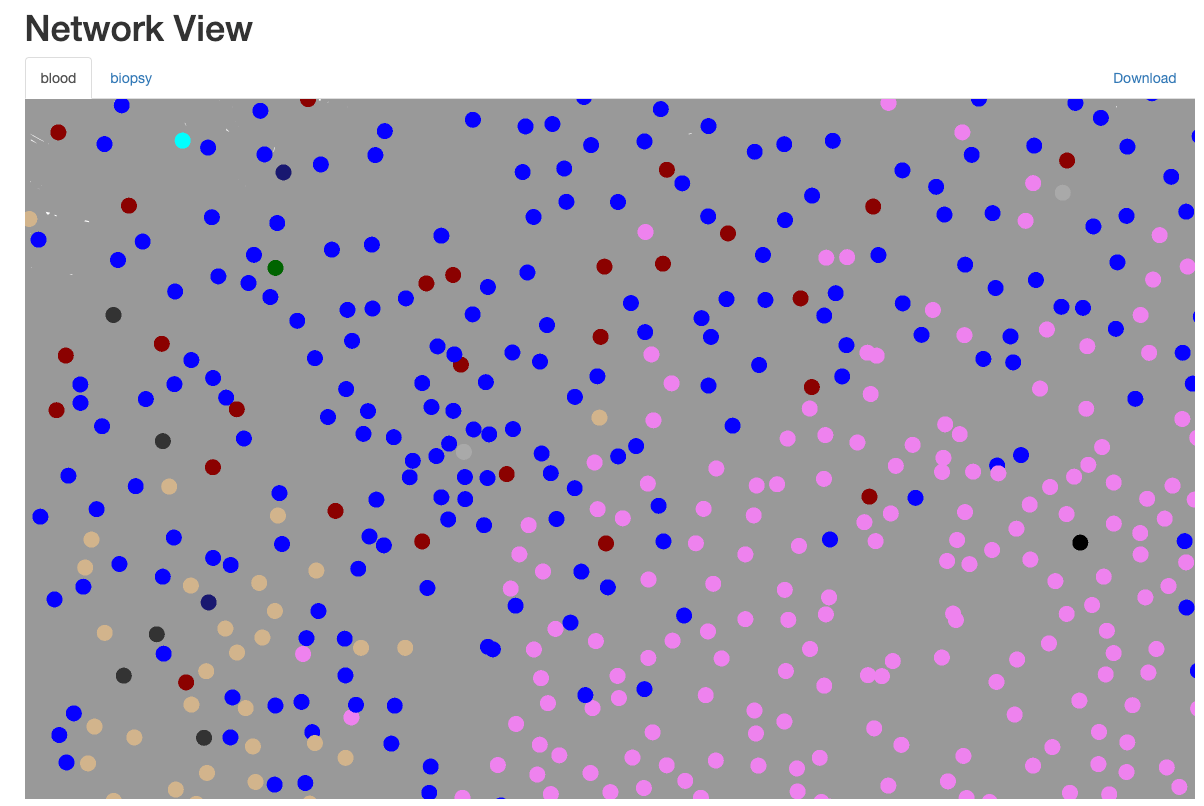
\includegraphics[width=\linewidth]{mixt_network2}
        \caption{Zoom in the network.}
        \label{fig:mixt_network_zoom}
    \end{subfigure}

    \caption{Network view of the MIxT application where nodes repsent genes and the modules are repsented by colors. Relationships are represented by grey lines that connect a gene with another one.}
    \label{fig:mixt_network}
\end{figure}

\section{Proposed solution and contribution}
We have built GeneNet VR, a Virtual Reality visualization system that focuses on solving the problem of visualization of networks with data overload in order to improve the discovery of novel patterns. We used the datasets from the MIxT project so that we work with realistic data sources. We applied Virtual Reality for the visualization and interaction with the networks and offer the following tools that differ from the visualization system built on MIxT:

\begin{itemize}
  \item 3-dimensional view of the network.
  \item Possibility to move around the virtual space to see the network from different angles.
  \item Application of 3-dimensional transformations to the network such as scaling and translation.
  \item Visualization of single node relationships.
  \item Possibility to filter the nodes using a user interface.
  \item Visualization of two networks at the same time in order to compare them in real time.
\end{itemize}

GeneNet VR results in an application that offers a different way for the visualization of biological networks and that gives visualization experts interesting tools to explore data. The application is also developed for Oculus Quest, a standalone VR headset, where we take the advanatage of visualizing the networks without the need of cables and a computer.

For the evaluation of GeneNet VR, we have focused on performance and scalability problems, which we consider important for the experts during the visualization process so that the identification of patterns doesn't get interrupted by slowliness and low FPS. We found out that the performance is good when visualizing datasets similar to the ones from MIxT in both PC and the Oculus Quest headset. As for future work, we would like to test GeneNet VR with larger datasets and with datasets from other fields that are not biology.

\section{Outline}

We have structured the thesis in the following chapters: Chapter 2 descibes how GeneNet VR was implemented, the architecture, design and the Virtual Reality techniques that were used. Chapter 3 focuses on explaining the visualization of MIxT in Virtual Reality. Chapter 4 describes some related projects found in the literature and we compare them with GeneNet VR. In Chapter 5 we describe the experimens and conclusions that carried out in order to evaluate GeneNet VR. In Chapter 6 we explain the conclusions from the project. In Chapter 7 we describe the future work ideas that we have for GeneNet VR.
